\section{Approach}

% draw two pics, one is overview, describing a detail example. from candidate generation, focus entity identification, and a basic siamese structure. The other one is detailed network structure of our schema encoding.
In this section, we describe our nerual network based model for KBQA. The architecture of our proposed model is shown in \figref{fig:overview}. First, we identify focus entity and generate candidate query graphs by searching paths with certain constraints in KB (\secref{sec:candgen}). Next we encode question and candidate query graph respectively. 
More specifically, we use a bi-directianl RNN structure to represent question (\secref{sec:q-encoding}) and a complex embedding strategy is employed to encode a complex query graph (\secref{sec:schema-encoding}). Then we propose a cross attention mechanism to measure the similarity between a question and a query graph (\secref{sec:attention}). Finally, we discuss the prediction and parameter learning step of this task (\secref{sec:training}).


\begin{figure*}
	\centering
	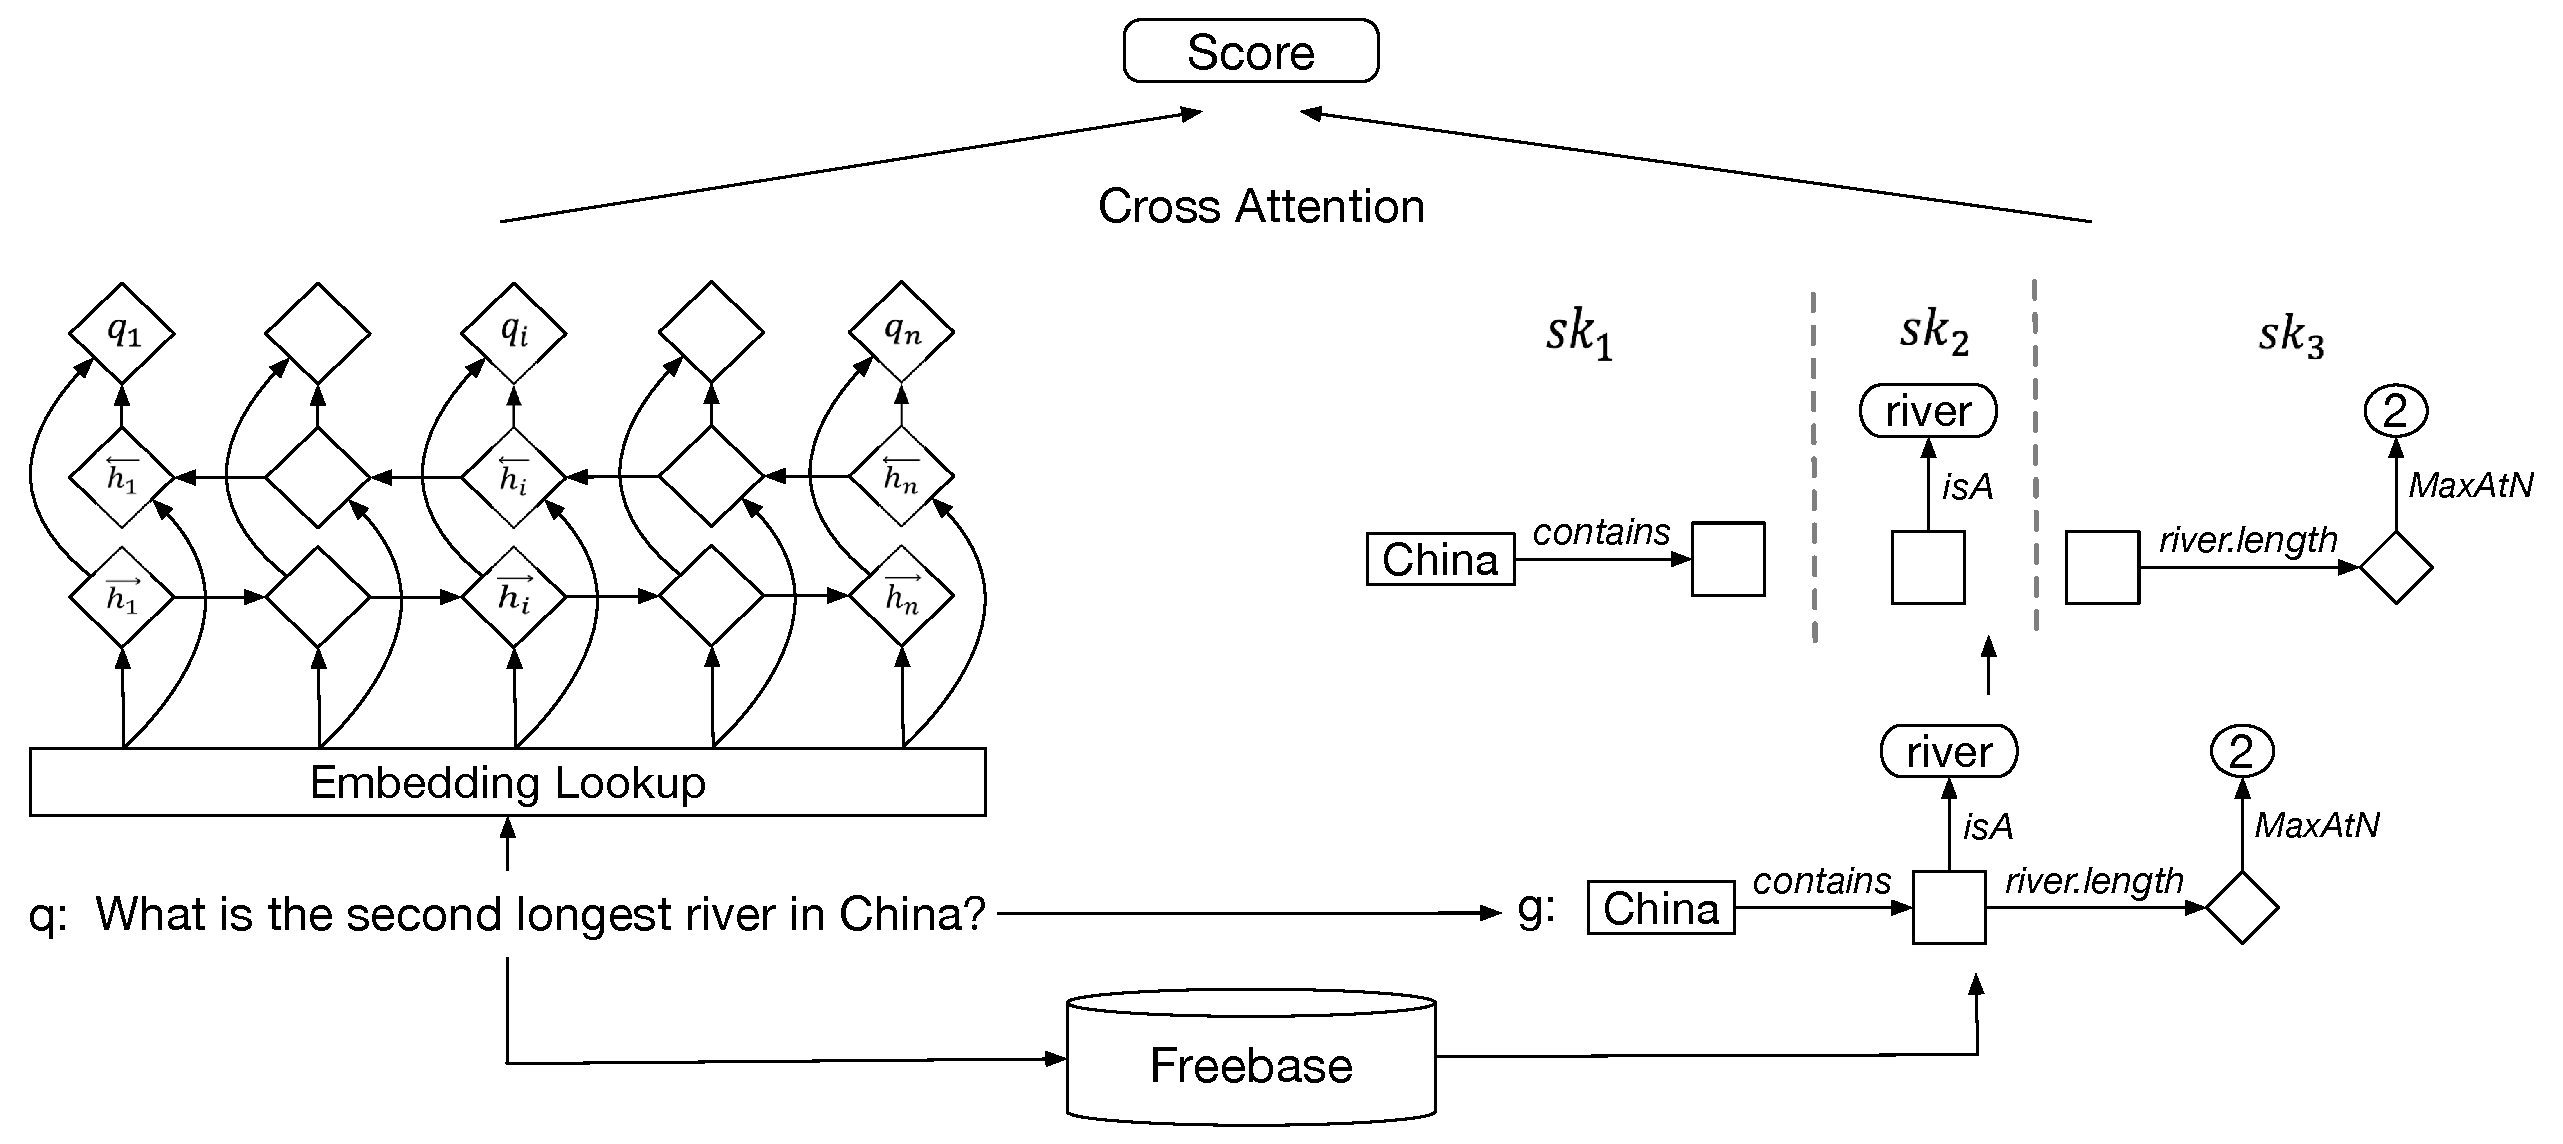
\epsfig{file=figures/overview.eps, angle=0, width=2.0\columnwidth}
	%\scalebox{0.3}{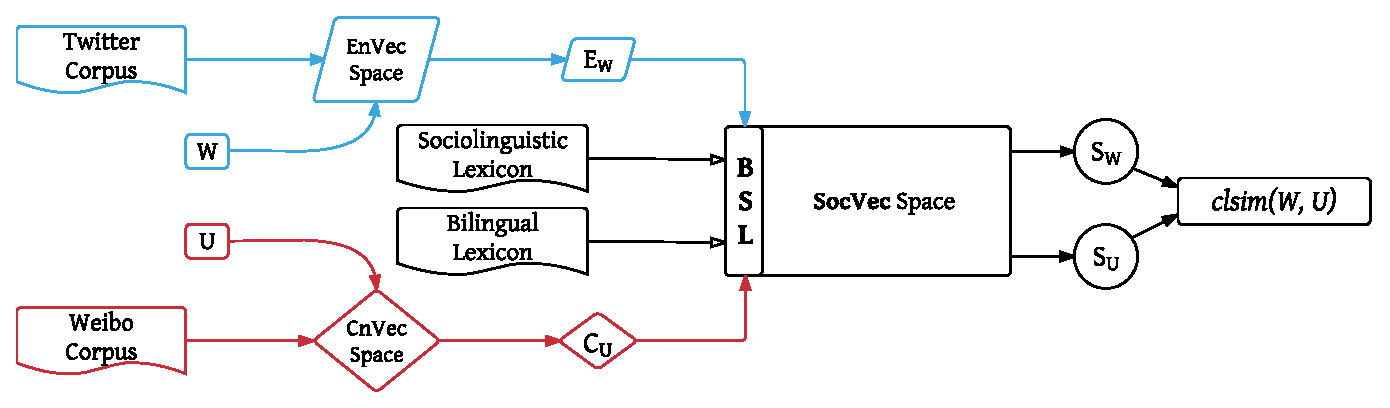
\includegraphics{overview.eps}}
	\caption{Overview of proposed neural network model.}
	\label{fig:overview}
\end{figure*}
 

\subsection{Candidate Generation}
\label{sec:candgen}


Given a question , it's a common practice to generate all candidate query structures through several
query stages~\cite{yih2015,bao2016}.
The main idea is to first find focus entites as the starting point of all query structures,
then extract main paths, and finally enrich the main path by adding different kinds of constraints.
Now we explain in detail the different querying stages.
%by performing SPARQL querys : generate main path first, and enrich add different kinds of constaints.
%Given a question, we    multiple stages.  (follow Bao and Yih)
%(need two detail figures showing the different parts)

\textbf{Focus Entity Generation.}
We use the S-MART entity linker~\cite{yang2015} to recognize possible entities in the question.
S-MART linker detects possible entity mentions (surface forms of phrases) which would map to entities in the knowledge base,
and score each (mention, entity) pair by a MART based on stat features, such as the lexical similarity,
link prob on Wiki and entity popularity in Wikipedia.
Following the S-MART results provided by Yih et al.~\shortcite{yih2015},
up to 10 top-ranked (mention, entity) pairs will be returned.
One mention could lead to several entities.
For example, the mention ``Star Trek'' links to several possible films in the result.

\textbf{Main Path and Entity Constraint Generation.} 
Given all possible focus entitie of the question, we first build the main path of the query structure.
We enumerate each entity as the main entity, and take the regard remaining as possible contraint entities.
We search the knowledge base and explore all 1-hop and 2-hop-with-med predicate sequences
starting from the main entity.
For example, ...
along this path, answer node could be xxxx and the intermediate entity are mediators describing the particular actor-film-starring fact.
Afterwards, we attempt to add entity constraints to the main paths.
%TODO: add SPARQL query example to the query structure
if the constraint entity can be linked to the answer entity or intermediate entity by some 1-hop predicates.
As the running example of Figure xxx, the constraint entity yyy is connected to the entity by the predicate "zzz".

\textbf{Type Constraint Generation.}
Type constraint is more restricted, where a candidate FB type is linked to only the answer node by ``type.object.type'' in FB.
Since S-MART doesn't provide information of type mentions, we propose a simple but effective method for detecting type mentions.
We enumerate all the N-gram surface forms of the question as candidate type mention, and calculate the cosine similarity
between the average word embedding of type mentions and the average embedding of type names in FB.
Similar with S-MART, we return up to 10 (mention, type) pairs.
In order to make the query structure consistent in semantics, we attempt to apply the type
constriant to the current query structure, if there are overlapping s between the type
and the range type of the main path.
Taking xx as example, the range is ``location'', therefore candidate type like ``river'' can be applied,
non-overlapping candidate types (like ``person'', ``book'') are discarded, if existed.
%TODO: Talk about topical consistent predicates.

\textbf{Time Constraint Geneartion.}
We extract time mention by simply matching year regex.
Different from the previous constraints, the preposition before the time mention is meaningful,
then we include it into the time mention.
Then we attampt to link the time to main paths through the "op+predicate" sequence.
the predicate is inplicit datetime predicates of the 
intermediate entity and answer node (including constraint types binding to the answer).
The preposition represents datetime comparison operators as lt, gt, within.

\textbf{Ordinal}
Similar with time constraint: finding mentions and link throught "op+predicate" sequence.
mention: ordinal words (``fist'', ``2nd'') and superlative words (``longest'', ``largest'').
We collect the set of superlative words which tends to describe factual and object attributes.
Therefore, the mention encodes both target ranks and the semantic of ordinal predicates.
The op are chosen from two virtual operators: max and min.
The predicate are topical consistent predicates whose range are int, float or datetime.
in order to control the size of cands brought by ordinal constraints,
leverage word embedding ,extract top-2 by calculating the cosine similarity
between mention embedding and predicate name embedding.

After all these querying stages, we collect a list of candidate structures at different granularity.
We translate into SPARQL query, resulting in the final answer of the query structures.
We filter out structures with 0 outputs, and structures which uses overlapping mentions.
Resulting in ~180 candidate structures per question.


%Given a question, we have to generate a set of query graphs with multiple complex constraints. In general, we first detect entities mentioned in the question. Then for each entity, we regard it as a fixed node and starting from it we search for a path in KB. A path is composed of at most two hop predicates. For example, the $\bi{sk}_1$ in the right part of \figref{fig:overview} is such a path with one hop predicate since ``China'' is an entity.

%However, basic path can only express the semantics of single relation question, but can not support a question with multiple complex constraints such as the one in \figref{fig:overview}. Thus, we have to add those complex constraints to the simple path to restrict the answer. There are four different constraints in our consideration, which are entity constraint, type constraint, temporal constraint and ordinal constraint. Entity constraint, 


\subsection{Question Representation}
\label{sec:q-encoding}


1. q definition
2. 

placeholder
positional embedding

Before the step of cross-attention, we encode the input questions as the distributional
representation of each word in it.
Specifically, the input question $q$ is expressed as the word sequence $q=(w_1, w_2, \dots, w_n)$,
where $w_i$ denotes the $i$-th word.
%TODO: trick of E and Tm
We first use a word embedding matrix $E_w \in \mathbb{R}^{|V_w| \times d}$ to convert 
the original sequence into word embeddings $\bi{q}=(\bi{w}_1, \bi{w}_2, \dots, \bi{w}_n)$,
where $|V_w|$ denotes the vocablary size of natural language words,
and $d$ denotes the embedding dimenson.
The word embedding matrix is initialized by publicly available pre-trained results, 
such as Word2vec~\cite{mikolov2013} and GloVe~\cite{xxx}. 

In the next step, we feed the word embeddings into a bidirectional Gated Recurrent Unit (GRU)~\cite{xxx} networks.
As a brief introduction, GRU is capable of effectively maintaining the long-distance dependency in many NLP tasks.
Given $\bi{x}_t$ as the input of time step $t$ of RNN, and $\bi{h}_{t-1}$ as the hidden state at time stamp $t-1$,
GRU calculates the current hidden state $\bi{h}_t$ through gated units, described in \eqnref{eqn:gru}:

\begin{equation}
  \label{eqn:gru}
  \begin{aligned}
    & \bi{r}_t & = & \sigma(\bi{W}_r\bi{x}_t+\bi{U}_r\bi{h}_{t-1}), \\
    & \bi{z}_t & = & \sigma(\bi{W}_z\bi{x}_t+\bi{U}_z\bi{h}_{t-1}), \\
    & \tilde{\bi{h}}_t & = &\mbox{tanh}(\bi{W}_h\bi{x}_t+\bi{U}_h(\bi{r}_t\cdot\bi{h}_{t-1})), \\
    & \bi{h}_t & = & (1-\bi{z}_t)\cdot\bi{h}_{t-1}+\bi{z}_t\cdot\tilde{\bi{h}}_t. \\
  \end{aligned}
\end{equation}

\noindent
In the case of GRU, the vector $\bi{r}_t$ is the output of the \textit{reset gate},
determining how much information of the last state $\bi{h}_{t-1}$ is ignored
in the computation of the candidate state $\tilde{\bi{h}}_t$.
The vector $\bi{z}_t$ is the output of the \textit{update gate}, which controls the interpolation 
between the last state $\bi{h}_{t-1}$ and the candidate state $\tilde{\bi{h}}_t$.

For encoding the input question, we employ the bidirectional GRU network, which consists a
forward network and a backward network encoding in the reverse order.
Taking the word embedding sequence $(\bi{w}_1, \dots, \bi{w}_n)$ as input,
we get the forward hidden sequence
$(\overrightarrow{\bi{h}_1}, \overrightarrow{\bi{h}_2}, \dots, \overrightarrow{\bi{h}_n})$ 
as well as the backward one
$(\overleftarrow{\bi{h}_1}, \overleftarrow{\bi{h}_2}, \dots, \overleftarrow{\bi{h}_n})$.
We concatnate the forward hidden state of each word with corresponding backward hidden state,
resulting in the distributional representation $\bi{h}^{(w)}_i = [\overrightarrow{\bi{h}_i};\overleftarrow{\bi{h}_i}]$.
Thus, we obtain the representation of each word in the question, and each hidden state
encodes the information from both before and after the corresponding word.




\subsection{Query Graph Representation}
\label{sec:schema-encoding}

After candidate generation, we obtain a set of candidate complex query graphs for each question $q$. A complex query graph $g$ can be regarded as a set of simple skeletons $(sk_1, sk_2, \dots, sk_m)$. We define a skeleton $sk$ is a predicate path starting from a fixed node to the target answer. The fixed starting node can be an entity, a type, a number, datetime or an ordinal value. Together with predicate, we call them ``items''. Thus we denote $sk = (it_1, it_2, \dots, it_l)$ (Note that this sequence has an order from starting point to target answer). In the case of \figref{fig:overview}, the candidate query graph in the right side can be splited into three skeletons, which start from ``entity:China'', ``type:River'' and ``ordinal$\_$value:$2$'' respectively. 
Now we describe in detail how to obtain the skeleton representation $\bi{sk}$ and further represent a complex query graph $g$ into $\bi{g} = (\bi{sk}_1, \bi{sk}_2, \dots, \bi{sk}_m)$. 

%1. item encoding
Firstly, we represent each component (item) of a skeleton into hidden vectors. For entity, type and predicate, we use their names in KB as text infomation and thus employ a bi-GRU network to encode the items just as we do in question encoding (\secref{sec:q-encoding}). For example, the name of entity ``China'' in \figref{fig:overview} is \textit{``People's Republic of China''} and we regard it as a word sequence [``people'', ``republic'', ``of'', ``China'']. After embedding lookup, the sequence of word embeddings are fed into bi-GRU, resulting a sequence of hidden vectors $[\overrightarrow{\bi{h}_i};\overleftarrow{\bi{h}_i}]$. Then we average them to obtain the item representation $\bi{it}$.

\begin{equation}
\label{eqn:item}
\begin{aligned}
& \bi{it} & = & \frac{1}{N}\sum_{i}[\overrightarrow{\bi{h}_i};\overleftarrow{\bi{h}_i}]\\
\end{aligned}
\end{equation}
\noindent
where $N$ is the number of words in that name.
For number, datetime and ordinal value, we add three special placeholders in word embedding vocabulary and initialize them randomly. Thus, these three items are represented directly through embedding lookup. 

%2. skeleton representation

Then, we represent a skeleton $\bi{sk}$ as a dynamic combination of its item representations $\bi{it}_i$ shown in \figref{fig:overview} (right side). Since the items of a skeleton also form into a sequence in order, we use another bi-GRU to encode item sequence.

Up to now, we have obtained the representation of query graph $\bi{g}$ consisting of a set of skeletion representations $(\bi{sk}_1, \bi{sk}_2, \dots, \bi{sk}_m)$.




\subsection{Attention Mechanism}
\label{sec:attention}

Attention mechanisms \cite{bahdanau2014neural,luong2015effective} have become an integral part of sequence modeling and transduction models in various nlp tasks, allowing better understanding sequential data. In this paper, we introduce a cross-attention mechanism between question and query graph, aiming to better justify thier compatibility.

Our cross-attention mechanism consists of two parts: query graph towards question part and question towards query graph part. Our goal is to find the best query graph from the candidate set. When we look at a question $\bi{q} = (\bi{q}_1, \bi{q}_2, \dots, \bi{q}_n)$ and a candidate query graph $\bi{g} = (\bi{sk}_1, \bi{sk}_2, \dots, \bi{sk}_m)$, we have to judge which parts of the query graph are more related to the question, since each skeleton of a graph describes one semantic aspect of the question. Besides, when we look at the query graph, we will reread the question to find out which words are more focused. Hao et al., \cite{hao2017end} also propose a cross-attention mechanism, aiming to select the best answer towards a question. However, their method does not calculate the attention values on both sides simultaneously, instead they do it in two steps and use an average of word representations in question to guide the attention of answer aspects. 

\begin{figure*}
	\centering
	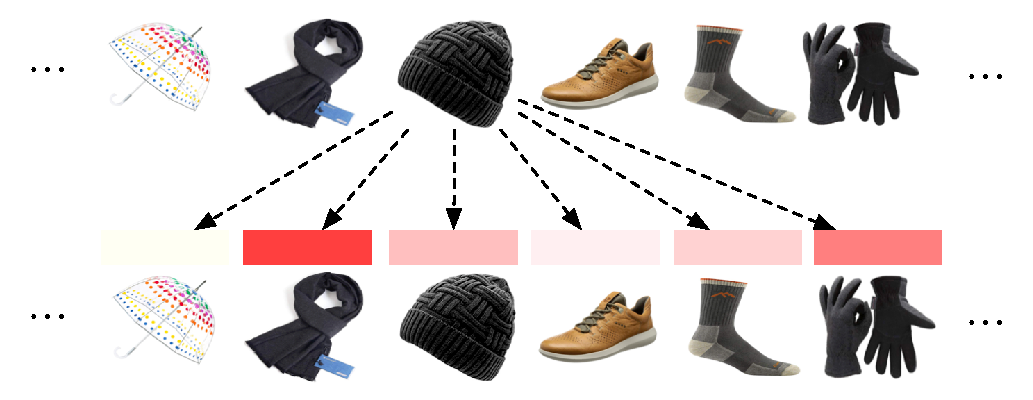
\epsfig{file=figures/attention.eps, angle=0, width=1.2\columnwidth}
	%\scalebox{0.5}{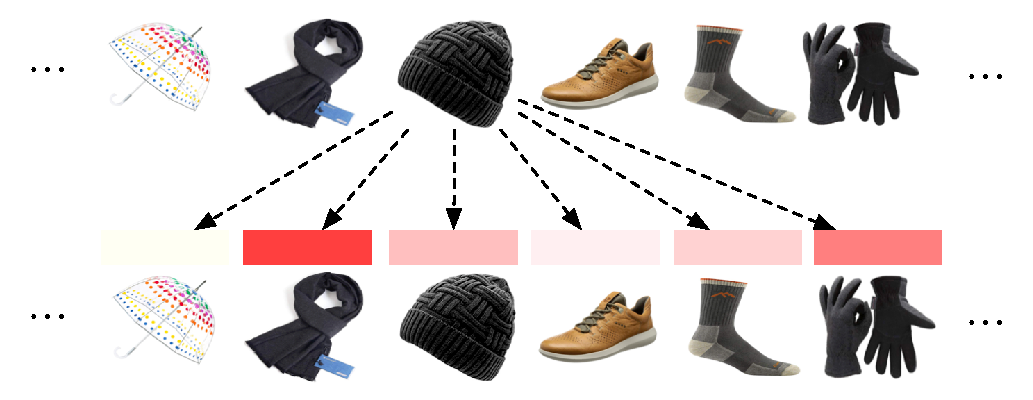
\includegraphics{figures/attention.eps}}
	\caption{Cross-attention architecture between question and query graph.}
	\label{fig:attention}
\end{figure*}

Inspired by ABCNN \cite{yin2015abcnn}, we propose a attention matrix $\bi{E}_{att}$  (\figref{fig:attention}), where the attention values of row $i$ denote the attention distribution of the $i$-th word in the question with respect to the query graph, and the attention values of column $j$ denote the attention distribution of the $j$-th skeleton in the query graph with respect to the question. Then we represents the whole question $\bi{q}$ and query graph $\bi{g}$ as follows. 




\begin{equation}
\label{eqn:att-q}
\begin{aligned}
& \bi{q} & = & \sum_{i}(\sum_{j}{\bi{E}_{att}}_{ij}) \times \bi{q}_i\\
\end{aligned}
\end{equation}
\noindent

\begin{equation}
\label{eqn:att-g}
\begin{aligned}
& \bi{g} & = & \sum_{j}(\sum_{i}{\bi{E}_{att}}_{ij}) \times \bi{sk}_j\\
\end{aligned}
\end{equation}
\noindent

In the end, we use a fully connected layer to get a similarity score between $\bi{q}$ and $\bi{g}$.



\subsection{Training and Prediction}
\label{sec:training}






